


\section{BERT (Bidirectional Encoder Representations from Transformers)}


\begin{frame}{BERT: Motivation}
    \normalsize 
    
    \begin{itemizeSpaced}{7pt}
        \item \textbf{Problem with ELMo: } shallowly combines ``independently-trained" biLMs
        
        \item \textbf{Problem with OpenAI GPT: }uses a left-to-right construction, where each token only attends to past tokens in the self attention layers of the Transformer $\Rightarrow$ cannot represent bidirectional context $\Rightarrow$ does poorly on \emph{sentence-level} and \emph{token-level} tasks (question answering (QA))

        
        \pinkbox \textbf{BERT's Solution: } train ``deep bidirectional representations from unlabeled text by jointly conditioning on both left and right context in all layers” (Devlin et al., 2019).
    \end{itemizeSpaced}
    
\end{frame}


\begin{frame}{BERT: Input Embeddings}
    \normalsize \linespread{0.5}
    
    \begin{enumerateSpaced}{15pt}
        \item \textbf{\textit{WordPiece} token embeddings: }The \emph{WordPiece} tokenization subdivides words to smaller units (instead of tokenizing by natural separations)
        
        \begin{itemizeSpaced}{15pt}
            \normalsize \linespread{0.5}
        
            \item to handle rare, unknown words (Weng, 2019) and reduce vocabulary size while increasing amount of data available per word.
            
            \item \textbf{Example: }if ``play" and ``**ing" and ``**ed" are present in the vocabulary but ``playing" and ``played" are not, then these can be recognized by their sub-units. 
        \end{itemizeSpaced}
        
        
        \item \textbf{Segment embeddings: } are arbitrary spans of text (packing sentence parts). 
        NOTE: Transformer-XL respects sentence boundaries. 
        
        \item \textbf{Positional embeddings: } as in ordinary Transformer (to inject word order information). 
    
    \end{enumerateSpaced}
    
\end{frame}




\begin{frame}{BERT Framework: MLM and NSP}

\linespread{0.3} 

BERT does \textbf{pre-training} (trains on \emph{unlabeled data} over different tasks), and \textbf{fine-tuning} (to use pre-training parameters to train over \emph{labeled data} for nlp tasks)

Pre-training involves:  \textbf{masked language modeling (MLM)} task and \textbf{next sentence prediction (NSP)} task to learn bidirectional context and \emph{sentence-level} information

Improvement over language models that just predict next tokens given context. 



{\large \textbf{Masked language model (MLM): }}
    \begin{itemizeSpaced}{2pt}
        \pinkbox \textbf{Motivation: } bidirectional conditioning causes information leakage (a word can implicitly ``see itself" letting the model trivially guess the target word in a multi-layered context (Devlin et al., 2019)). 
        
        \item \textbf{Goal: }randomly masks some input tokens to predict original masked word using only its context. 
        
        \item \textbf{Effect of MLM: } fuses left and right context to get \emph{deep} bidirectional context (unlike ELMo's shallow left-to-right language model (Devlin et al., 2019)).  
    \end{itemizeSpaced}
    
{\large \textbf{Next Sentence Prediction (NSP: }}
    \begin{itemizeSpaced}{2pt}
        \pinkbox \textbf{Motivation: }Ordinary  language models lack \emph{sentence-level} information $\Rightarrow$ cannot do well in question-answering (QA) and natural language inference (NLI) tasks
        
        
        \item \textbf{Goal: } task that finds if sentence is the next sentence of the other. 
        
    \end{itemizeSpaced}
    
\end{frame}


\begin{frame}{BERT: General Experimental Results}

    \begin{itemizeSpaced}{2pt}
        \item Using a simple accuracy measure, Munikar et al. (2019) found that a pre-trained BERT model fine-tuned for \textbf{sentiment analysis (SA)} task outperformed complex models (RNN, CNNs).
        
        \pinkbox This proves \textbf{transfer learning} is possible with BERT's deep contextual bidirectional language model. 
    \end{itemizeSpaced}



    \begin{table}[ht!]
      \centering
      \vspace{-7pt}
      
      \begin{tabular}{ c }
      
        \begin{minipage}{.7\textwidth}
          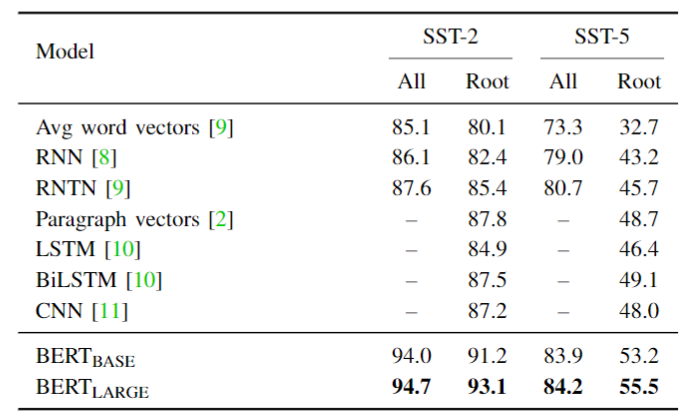
\includegraphics[width=\linewidth]{imgs/table_bert_vsOtherModels.png}
        \end{minipage}
        \vspace{-7pt}
      
      \end{tabular}
      
      \caption{\linespread{0.3} \footnotesize Accuracy (\%) of several models on \textbf{sentiment classification (SC)} SST dataset. BERT has highest accuracy scores. From \emph{Table B.II in Fine-Grained Sentiment Classification Using BERT}, by Munikar et al., 2019. \url{https://arxiv.org/pdf/1910.03474.pdf}. Copyright 2019 by Munikar et al.}
      \label{tbl:bertExperimentResults}
      \vspace{-10pt}
    \end{table}
    
\end{frame}



\begin{frame}{Probing BERT: BERT Learns Dependency Syntax}


    \begin{columns}
    
        \begin{column}{0.6\textwidth}
            \vspace{\topsep}
            
            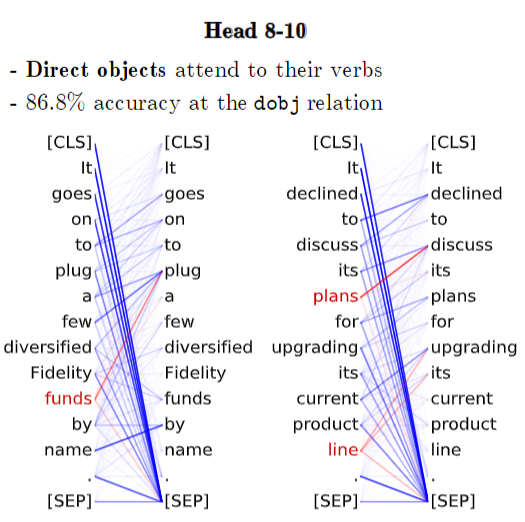
\includegraphics[width=0.8\columnwidth]{imgs/bert_headsDirectObject.png}
            
            \vspace{-5pt}
            
            \captionof{figure}{\linespread{0.3}\footnotesize BERT attention heads capture syntax. In heads 8-10, direct objects are found to attend to their verbs. Line darkness indicates attention strength. Red indicates attention to/from red words, to highlight certain attentional behaviors. From \emph{What Does BERT Look At? An Analysis of BERT's Attention}, by Clark et al., 2019. \url{https://arxiv.org/abs/1906.04341}. Copyright 2019 by Clark et al.} 
            \label{fig:bertHeadDirectObject}
        \end{column}
        
        \begin{column}{0.4\textwidth}
        
            Clark et al. (2019) found ...
            
            \begin{itemizeSpaced}{2pt}
            
                \item  While BERT's attention heads do not capture syntax dependency structure as a whole....
            
                \item ... different heads are better at detecting different syntax dependency relationships.
                
                \item \textbf{Example: }the heads detect ``direct objects of verbs, determiners of nouns, objects of prepositions, and objects of possessive pronouns with > $75 \%$ accuracy."
                
                \item Attention heads 8-10 in \cref{fig:bertHeadDirectObject} learn how direct objects attend to their verbs. 
                
                \item BERT learns this using only \textit{self-supervision}. 
            \end{itemizeSpaced}
        \end{column}
    
    \end{columns}


\end{frame}





\begin{frame}{Probing BERT: BERT's Limitation in Segment Representation}
    \normalsize
    \linespread{0.4}
    
    \begin{itemizeSpaced}{10pt}
        \item BERT does not use separator tokens (\texttt{[SEP]}) to gather segment-level information. 
        
        \pinkbox BERT uses \texttt{[SEP]} as ``no-op" or stub operations for attention heads when the head is not needed for a current task. 
        
        \item How? Why? Authors investigated in two ways ...
        
        \begin{itemizeSpaced}{10pt}
        
        \normalsize \linespread{0.4}
        
            \item If this were true, attention heads processing \texttt{[SEP]} should attend broadly over entire segment to make the segment vectors. BUT in \cref{fig:bertHeadDirectObject}, heads 8-10 direct objects attend to their verbs, and all other words attend to the \texttt{[SEP]} token. 
            
            \item Gradient measures: show much the attention to a token would change BERT's outputs. Attention to \texttt{[SEP]} increases in layers 5-10 (\cref{fig:bertSEPAttention}), WHILE the gradients for attention to \texttt{[SEP]} decrease here (\cref{fig:bertGradient})  $\Rightarrow$ attending to \texttt{[SEP]} does not significantly change BERT's outputs. 
        \end{itemizeSpaced}
    \end{itemizeSpaced}
    


So, BERT's attention heads attend to \texttt{[SEP]} when they have no other job, not to gather segment-level information. 

\textbf{Transformer-XL} by design improves this.

\end{frame}





\begin{frame}{(continued) Probing BERT: BERT's Limitation in Segment Representation}

    \begin{figure}
    \centering
    \begin{minipage}{.47\textwidth}
      \centering
      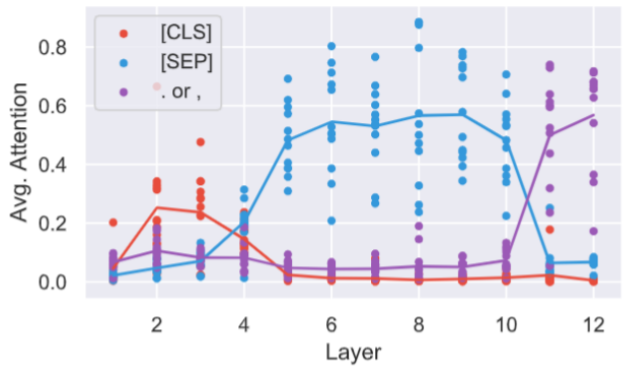
\includegraphics[width=\textwidth]{imgs/bert_attentionSEP_singleimage.png}
      \captionof{figure}{\linespread{0.3}\footnotesize BERT's attention heads in layers 6-10 spend more than half the average attention to separator tokens; deep heads attend to punctuation, while middle heads attend to \texttt{[SEP]}, and early heads attend to \texttt{[CLS]}. From \emph{What Does BERT Look At? An Analysis of BERT's Attention}, by Clark et al., 2019. \url{https://arxiv.org/abs/1906.04341}. Copyright 2019 by Clark et al.}
      \label{fig:bertSEPAttention}
    \end{minipage} \hspace{2em}%
    \begin{minipage}{.47\textwidth}
      \centering
      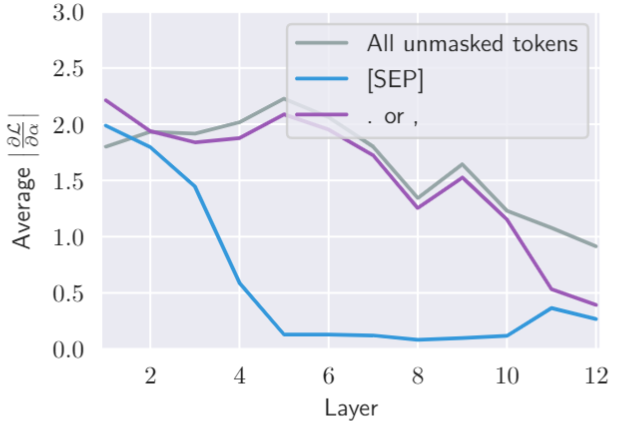
\includegraphics[width=\textwidth]{imgs/bert_attentionheads_gradient.png}
      \captionof{figure}{\linespread{0.3}\footnotesize Gradient-based estimates for attention to separator and punctuation tokens. Authors ``compute the magnitude of the gradient of the loss from the masked-language model (MLM) task with respect to each attention weight." From \emph{What Does BERT Look At? An Analysis of BERT's Attention}, by Clark et al., 2019. \url{https://arxiv.org/abs/1906.04341}. Copyright 2019 by Clark et al.}
      \label{fig:bertGradient}
    \end{minipage}
    \end{figure}

    
\end{frame}



\begin{frame}{BERT's Attempt at Polysemy}
    
    \begin{itemizeSpaced}{15pt}
    \linespread{0.3}
        \item Wiedemann et al. (2019) compared the contextual embeddings (CWE)s of ELMo and BERT on \textbf{word sense disambiguation (WSD)} task $\Rightarrow$ BERT places polysemic words into distinct regions according to their senses, while ELMo cannot (stronger word sense separation in BERT embeddings). 
        
        \item BERT did well when the text had ...
        \begin{itemizeSpaced}{7pt}
        \linespread{0.3}
            \item \textit{vocabulary overlap} {``along the bank of the river” (input text) and ``along the bank of the river Greta” (nearest neighbor found by BERT)}. 
            
            \item \textit{semantic overlap} {``little earthy bank” (input) and ``huge bank [of snow]” (nearest neighbor found by BERT)}
        \end{itemizeSpaced}
        
        \item BERT struggled when text had \emph{vocabulary and semantic overlap at the same time}
        \begin{itemizeSpaced}{7pt}
            \linespread{0.3}
            \item \underline{False prediction 1}: BERT predicted ``land bank" as in a \emph{supply or stock} while the correct sense of ``land bank" was \emph{financial institution}
            
            \item \underline{False prediction 2}: correct word sense of ``balloon" is a verb while BERT predicted a noun sense, so it did not even get the word class correct.
            
            \item \underline{False prediction 3}: correct sense label of the polysemic word ``watch" was \emph{to look attentively} while BERT predicted its sense as \emph{to follow with the eyes or the mind; observe}. 
        \end{itemizeSpaced}
        
    \end{itemizeSpaced}
    
\end{frame}